\chapter{Revisão Bibliográfica}

Para realização da revisão bibliográfica foram utilizados as ferramentas de buscas de artigos científicos do \textit{Google Scholar} (\url{https://scholar.google.com/}), \textit{IEEE Xplore} (\url{https://ieeexplore.ieee.org/Xplore/home.jsp}), \textit{ScienceDirect} (\url{https://www.sciencedirect.com/}) e \textit{Semantic Scholar} (\url{https://www.semanticscholar.org/}).

Como palavras-chaves na busca foram utilizados termos em inglês, sendo eles, \textit{"semantic similarity between texts"}, \textit{"measure degree of paraphrase"}, \textit{"paraphrase detection"}, \textit{"natural language processing"}, \textit{"measure semantic similarity between answers"} e \textit{"evaluation of descriptve answers"}. Os termos que trouxeram os melhores resultados e estavam presentes nos melhores artigos selecionados foram \textit{"semantic similarity"}, \textit{"natural language processing"} e \textit{"evaluation of descriptve answers"}.

Inicialmente foram selecionados 26 artigos que poderiam ser relevantes para o presente trabalho com base nos temas, a sumarização dos artigos pode ser vista na Tabela \ref{table:1} em que os artigos selecionados no final estão destacados na cor cinza.

% Please add the following required packages to your document preamble:
% \usepackage{booktabs}
% \usepackage{graphicx}
\begin{table}[htb!]
\centering
\resizebox{\columnwidth}{!}{%
\begin{tabular}{@{}lll@{}}
\toprule
\textbf{Título} & Fonte & Referência \\ \midrule
Determining Degree of Relevance of Reviews Using a Graph-Based Text Representation & IEEE & \cite{DeterminingDegreeRelevanceReviewsUsingGraphBasedTextRepresentation} \\
A Chinese text paraphrase detection method based on dependency tree & IEEE & \cite{ChineseParaphraseDetectionBasedDependencyTree} \\
Nowhere to Hide: Finding Plagiarized Documents Based on Sentence Similarity & IEEE & \cite{FindingPlagiarizedDocumentsBasedSentenceSimilarity} \\
Enhanced Text Matching Based on Semantic Transformation & IEEE & \cite{EnhancedTextMatchingBasedSemanticTransformation} \\
Semantic similarity based assessment of descriptive type answers & IEEE & \cite{SemanticSimilarityBasedAssessmentDescriptiveTypeAnswers} \\
A comparative analysis of various approaches for automated assessment of descriptive answers & IEEE & \cite{comparativeAnalysisVariousApproachesAutomatedAssessmentDescriptiveAnswers} \\
A reliable approach to automatic assessment of short answer free responses & SSL & \cite{ReliableApproachAutomaticAssessmentShortAnswerFreeResponses}  \\
A Descriptive Answer Evaluation System Using Cosine Similarity Technique & IEEE & \cite{DescriptiveAnswerEvaluationSystemUsingCosineSimilarityTechnique} \\
An Intelligent System for Evaluation of Descriptive Answers & IEEE & \cite{IntelligentSystemEvaluationDescriptiveAnswersFuzzyGraphs} \\
Application Research of Similarity Algorithm in the Design of English Intelligent Question Answering System & IEEE & \cite{ApplicationResearchSimilarityAlgorithmDesignEnglishIntelligentQuestionAnsweringSystem} \\
Near duplicate text detection using graph depiction & IEEE & \cite{NearDuplicateTextDetectionKendalRankCorrelationModelTVM} \\
Recognition of Parallelism Sentence Based on Recurrent Neural Network & IEEE & \cite{RecognitionParallelismSentenceBasedRecurrentNeuralNetwork} \\
LSGC: An Interactive Text Matching Model Combined with Enhanced Encoding & IEEE & \cite{LSGCInteractiveTextMatchingModelEnhancedEncoding} \\
A software system for determining the semantic similarity of short texts in Serbian & IEEE & \cite{SoftwareSystemSemanticSimilarityShortTextSerbian} \\
Arabic Semantic Textual Similarity Identification based on Convolutional Gated Recurrent Units & IEEE & \cite{ArabicSemanticTextualSimilarityConvolutionalGatedRecurrentUnits} \\
A Chinese text paraphrase detection method based on dependency tree & IEEE & \cite{ChineseParaphraseDetectionBasedDependencyTree} \\
Using paraphrases to improve tweet classification: Comparing WordNet and word embedding approaches & IEEE & \cite{UsingParaphrasesTweetClassificationComparingWordNetAndWordEmbedding} \\
\rowcolor{Gray} SemEval-2020 Task 1: Unsupervised Lexical Semantic Change Detection & SSL & \cite{UnsupervisedLexicalSemanticChangeDetection} \\
SemEval-2017 Task 1: Semantic Textual Similarity Multilingual and Crosslingual Focused Evaluation & SSL & \cite{SemanticTextualSimilarityMultilingualCrosslingualFocusedEvaluation} \\
\rowcolor{Gray} Use of Syntactic Similarity Based Similarity Matrix for Evaluating Descriptive Answer & IEEE & \cite{SyntacticSimilarityBasedSimilarityMatrixForEvaluatingDescriptiveAnswer} \\
\rowcolor{Gray} Chapter 16 - Semantic similarity–based descriptive answer evaluation & SCD & \cite{SemanticSimilarityBasedDescriptiveAnswerEvaluation} \\
\rowcolor{Gray} A Study of Automated Evaluation of Student’s Examination Paper using Machine Learning Techniques & IEEE & \cite{StudyAutomatedEvaluationStudentsExaminationPaperMachineLearningTechniques} \\
Online Examination with short text matching & IEEE & \cite{OnlineExaminationWithShortTextMatching} \\
Towards Automated Evaluation of Handwritten Assessments & IEEE & \cite{TowardsAutomatedEvaluationHandwrittenAssessments} \\
Automatic Short Answer Grading (ASAG) using Attention-Based Deep Learning MODEL & IEEE & \cite{AutomaticShortAnswerGrading-ASAG-usingAttentionBasedDeepLearningMODEL} \\
Semantic similarity–based descriptive answer evaluation & SSL & \cite{SemanticSimilarityBasedDescriptiveAnswerEvaluation} \\ \bottomrule
\end{tabular}%
}
\caption{Tabela de revisão bibliográfica sumarizada.}
\label{table:1}
\end{table}


%\begin{figure}
%    \centering
%    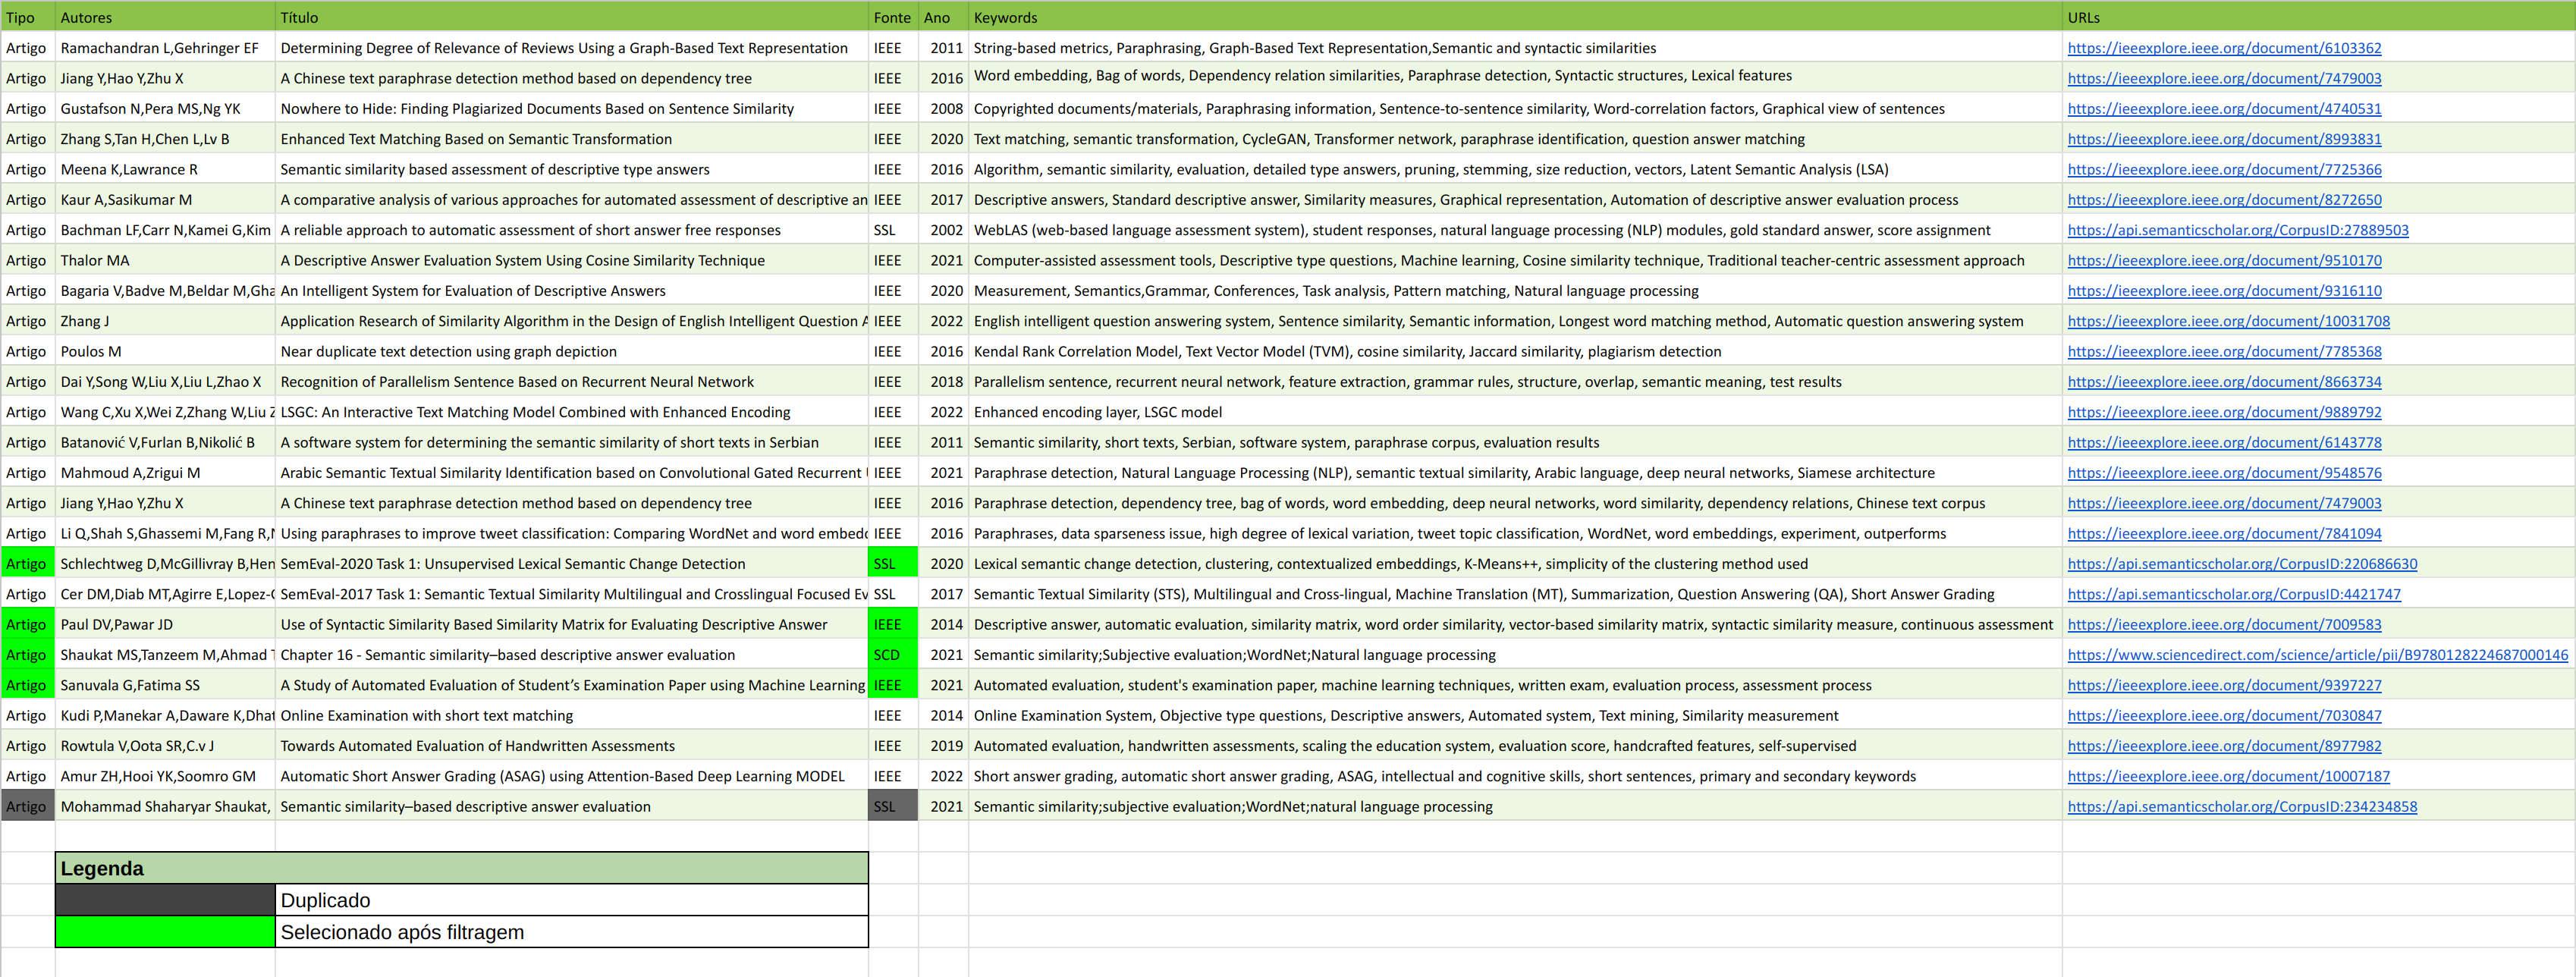
\includegraphics[width=\textwidth]{imgs/rev.png}
%    \caption{Figura da tabela de revisão bibliográfica sumarizada.}
%    \label{fig:1}
%\end{figure}

Após uma filtragem com base nos resumos e palavras-chaves, tendo como critério, a semelhança dos termos e a similaridade de outros artigos em comparação com a proposta do presente artigo, foram selecionados quatro artigos como base para a revisão bibliográfica como consta na Tabela \ref{table:2}, para leitura integral de seu conteúdo.

\begin{table}[htb!]
\resizebox{\columnwidth}{!}{%
\begin{tabular}{@{}lrrrr@{}}
\toprule
\textbf{Base} &
  \multicolumn{1}{l}{Total encontrados} &
  \multicolumn{1}{l}{Após remoção dos Duplicados} &
  \multicolumn{1}{l}{Após análise do resumo} \\ \midrule 
IEEE             & 21 & 21 & 2 \\
Science Direct   & 1  & 1  & 1 \\
Semantic Scholar & 4  & 3  & 1 \\ \bottomrule
\end{tabular}%
}
\caption{Tabela do funil de leitura.}
\label{table:2}
\end{table}

\newpage

O artigo proposto por \cite{UnsupervisedLexicalSemanticChangeDetection}, faz o uso de \textit{embeddings} de tipo (\textit{type embeddings}) e \textit{embeddings} contextualizados (\textit{token embeddings}) para representar as palavras. Primeiro, é introduzida a distribuição de frequência de sentido (SFD), e a detecção de mudança binária é definida em termos de limiares de frequência. Após isso, a distância de Jensen-Shannon (JSD) entre as distribuições normalizadas de frequência é utilizada para medir a mudança efetuada.
    
No artigo proposto por \cite{SyntacticSimilarityBasedSimilarityMatrixForEvaluatingDescriptiveAnswer}, podemos destacar que o trabalho utiliza a técnica de Análise Semântica Latente (LSA), que é comumente usada para determinar a similaridade de documentos, mas ressalta suas limitações em documentos curtos. O artigo destaca a ausência de abordagens anteriores que se concentrem na avaliação automática de respostas descritivas usando vetores de ordem de palavras. O método proposto utiliza uma matriz de similaridade entre vetores de ordem de palavras para avaliar respostas descritivas. A similaridade entre os vetores é calculada por meio de uma métrica de similaridade sintática, ou seja baseada na ordem das palavras. Os resultados indicam que a abordagem baseada em ordem de palavras é promissora para a avaliação automática de respostas descritivas. A matriz de similaridade é apresentada como uma ferramenta eficaz para computar as notas de cada pergunta.
    
Na proposta do artigo escrito pelos autores \cite{SemanticSimilarityBasedDescriptiveAnswerEvaluation}, pode-se destacar que a pesquisa faz uso de Processamento de Linguagem Natural (NLP) para automatizar o processo de avaliação, especialmente a similaridade de cosseno e índices de similaridade, são empregadas para atribuir notas às respostas.
    
Os autores \cite{StudyAutomatedEvaluationStudentsExaminationPaperMachineLearningTechniques} incorporam uma abordagem que emprega ferramentas de Reconhecimento Óptico de Caracteres (OCR) para extrair texto de respostas manuscritas digitalizadas. A ênfase principal, no entanto, recai sobre o emprego de técnicas avançadas de processamento de linguagem natural para aprimorar a avaliação. O estudo destaca a importância de etapas como a tokenização, remoção de stop words e verificação de sinônimos e antônimos no pré-processamento das respostas. Além disso, aborda a criação de modelos semânticos e o cálculo de similaridade sem mencionar explicitamente as métricas de Machine Learning utilizadas.



No contexto da revisão bibliográfica, alguns conceitos importantes foram retirados dos artigos selecionados, para contribuir com o presente trabalho. Dentre esses, destacam-se a análise da similaridade semântica com cossenos, a consideração da frequência de Sentidos de Palavras (SFD) e a utilização de vetores de ordem de palavras como elementos-chave.

A análise de similaridade semântica com cossenos é uma técnica importante, conforme evidenciado nos artigos revisados \cite{SemanticSimilarityBasedDescriptiveAnswerEvaluation}. Essa abordagem é frequentemente empregada para medir a proximidade semântica entre textos.

O uso da Frequência de Sentidos de Palavras (SFD) em um dos artigos indica a importância específica da distribuição de frequência das palavras. Esse conceito pode contribuir para o trabalho, sendo relevante para aspectos da sintaxe e da semântica do texto.

A utilização de vetores de ordem de palavras, como abordado em um dos artigos, resalta a importância da ordem das palavras na avaliação de respostas descritivas. Essa técnica pode superar limitações associadas à Análise Semântica Latente (LSA) em documentos curtos, oferecendo uma abordagem promissora para a avaliação automática.

Em síntese, a revisão bibliográfica gerou a necessidade de explicitar conceitos fundamentais a análise de similaridade semântica com cossenos, a distribuição de frequência de sentidos de palavras e da exploração de vetores de ordem de palavras como pontos relevantes nos estudos revisados.

\newpage